\documentclass[a4paper,12pt,dutch]{article}
\usepackage{glossaries}
\usepackage[T1]{fontenc}
\usepackage{babel}
\usepackage{graphicx}
\usepackage[table,xcdraw]{xcolor}
\usepackage{hyperref}
\usepackage{blindtext}
\usepackage{geometry}
\usepackage{parskip}
\usepackage{mathtools}
\usepackage{siunitx}
\usepackage{listings}
\usepackage{csquotes}
\usepackage{caption}
\usepackage{subcaption}
\usepackage{comment}
\usepackage{pdfpages}
\usepackage{pict2e}

% \DeclareRobustCommand{\slashcirc}{{\mathpalette\doslashcirc\relax}}

% \makeatletter
% \newcommand\doslashcirc[2]{%
%   \sbox\z@{$#1\m@th\circ$}%
%   \setlength\unitlength{\wd\z@}
%   \begin{picture}(1,1)
%   \roundcap
%   \put(0,0){\box\z@}
%   \put(0,0){\line(1,1){1}}
%   \end{picture}%
% }
% \makeatother


% %% Some packages you will need
% \usepackage{pgfplots}
% \usepackage{pgfplotstable}
% \usepackage{booktabs}
% \usepackage{array}
% \usepackage{colortbl}


\definecolor{arduinoorange}{HTML}{FFA500}
\definecolor{arduinogray}{HTML}{808080}
\definecolor{arduinoblue}{HTML}{007ACC}
\definecolor{arduinogreen}{HTML}{469B00}

\lstset{
  language=C++,
  basicstyle=\ttfamily\footnotesize,
  keywordstyle=\color{arduinoorange},
  stringstyle=\color{arduinogreen},
  commentstyle=\color{arduinogray},
  moredelim=[s][\color{arduinoblue}]{\#}{\ },
  morekeywords={digitalRead,digitalWrite,pinMode,analogRead,analogWrite,Serial,begin,HIGH,LOW},
  frame=tb,
  tabsize=4,
  showstringspaces=false,
  breaklines=true,
  numbers=left,
  numberstyle=\tiny\color{arduinogray},
  numbersep=5pt,
  extendedchars=true,
  literate={á}{{\'a}}1 {ã}{{\~a}}1 {é}{{\'e}}1,
}

\lstdefinestyle{Arduino}
{
  language=C++,
  basicstyle=\ttfamily\footnotesize,
  keywordstyle=\color{arduinoorange},
  stringstyle=\color{arduinogreen},
  commentstyle=\color{arduinogray},
  moredelim=[s][\color{arduinoblue}]{\#}{\ },
  morekeywords={digitalRead,digitalWrite,pinMode,analogRead,analogWrite,Serial,begin},
  frame=tb,
  tabsize=4,
  showstringspaces=false,
  breaklines=true,
  numbers=left,
  numberstyle=\tiny\color{arduinogray},
  numbersep=5pt,
  extendedchars=true,
  literate={á}{{\'a}}1 {ã}{{\~a}}1 {é}{{\'e}}1,
  backgroundcolor=\color{black!85},
  rulecolor=\color{arduinoorange},
  frame=single,
  frameround=tttt,
  framexleftmargin=6pt,
  framexrightmargin=6pt,
  framextopmargin=6pt,
  framexbottommargin=6pt,
  breaklines=true,
  postbreak=\raisebox{0ex}[0ex][0ex]{\ensuremath{\color{red}\hookrightarrow\space}},
}

\usepackage[
    backend=biber,
    backref=true,
    backrefstyle=none,
    sortcites=true,
    sorting=none,
    doi=false, % doi informatie wordt niet weergegeven
    %uniquename=true,
    %uniquelist=true,
    maxcitenames=3,
    %issn=false, werkt niet
    language=american
]{biblatex}
\addbibresource{information/Sources.bib}
\DefineBibliographyStrings{dutch}{
    backrefpage = {blz.},
    backrefpages = {blz.},
}
\makeglossaries
\definecolor{Grey1}{HTML}{343434}
\graphicspath{{./Media/Figuren/}}
 \geometry{
 a4paper,
 total={170mm,257mm},
 left=20mm,
 top=20mm,
 }
\hypersetup{
    colorlinks=true,
    linkcolor=blue,
    filecolor=magenta,      
    urlcolor=cyan,
    pdftitle={Overleaf Example},
    pdfpagemode=FullScreen,
    }


\begin{document}
\title{
\includegraphics[width=7in]{img/TraccyNew.jpg} \\
\vspace*{0.8in}
\textbf{Trap verlichting}\\
\textit{Plan van aanpak}\\
Versie 1
}
\author{
\vspace*{0.2in} \\
  Geschreven door:\\
  Laurens van der Drift\\
  Tommy Dobos\\
  Marnix Harmsen\\
  Luuk van Kappel\\
\vspace*{0.2in} \\
    Traccy Solutions\\
    \textbf{1892 Eten \& Drinken}\\
    Zoetermeer, Nederland
   } 
\maketitle
\phantomsection
\section*{Versie geschiedenis} \addcontentsline{toc}{section}{Versie geschiedenis}

\begin{table}[h]
\begin{tabular}{|l|l|l|l|}
\hline
\rowcolor[HTML]{4472C4} 
{\color[HTML]{FFFFFF} \textbf{Versie}} &
  {\color[HTML]{FFFFFF} \textbf{Datum}} &
  {\color[HTML]{FFFFFF} \textbf{Verandering}} &
  {\color[HTML]{FFFFFF} \textbf{Auteur}} \\ \hline
\rowcolor[HTML]{D9E1F2} 1.0 & \multicolumn{1}{c|}{\cellcolor[HTML]{D9E1F2}11-04-2024} & N.v.t. & Traccy Solutions \\


% \rowcolor[HTML]{FFFFFF} 
% 2.0 &
%   \multicolumn{1}{c|}{\cellcolor[HTML]{FFFFFF}7-4-2023} &
%  Feedback van FeedbackFruits toegepast &
%   Infra   Vroom \\ \hline

% \rowcolor[HTML]{D9E1F2} 
% 3.0 &
%   \multicolumn{1}{c|}{\cellcolor[HTML]{D9E1F2}4-6-2023} &
%  Bijgewerkt voor Assessment 3 &
%   Infra   Vroom \\ \hline

\end{tabular}
\end{table}
% %\addcontentsline{toc}{section}{Verklarende Woordenlijst}
\printglossaries
\newglossaryentry{tender}
{
    name=\textit{tender},
    description={De inschrijving om op een kavel een wind turbine park te bouwen.}
}

% \include{information/ListOfFigures}
\include{main/TableOfContents}
\section{Het probleem:}
Onder de trappen is er onvoldoende verlichting, waardoor de treden niet goed zichtbaar zijn voor alle gasten. Dit gebrek aan zichtbaarheid kan leiden tot mogelijke ongelukken en letsel. Daarnaast heeft 1892 Eten \& Drinken aangegeven dat er behoefte is aan decoratie onder de bar om de sfeer te verbeteren en de ruimte aantrekkelijker te maken voor de gasten.

\subsection{De opdracht}
Traccy Solutions heeft de opdracht gekregen om de verlichting onder de trappen en bar aan te leggen bij 1892 Eten \& Drinken. Dit omvat het installeren van LED-strips met adresseerbare LED's om aantrekkelijke effecten te creëren die de ambiance van de zaal versterken en de kans op letsel te verkleinen. Deze verlichting zal worden aangestuurd via een speciale app voor een intuïtieve bediening.

\begin{figure}[!h]
\centering
\begin{subfigure}{.5\textwidth}
  \centering
  \includegraphics[width=.5\linewidth]{img/1892_trap.jpg}
  \caption{De trap in de huidige staat.}
  \label{fig:sub1}
\end{subfigure}%
\begin{subfigure}{.5\textwidth}
  \centering
  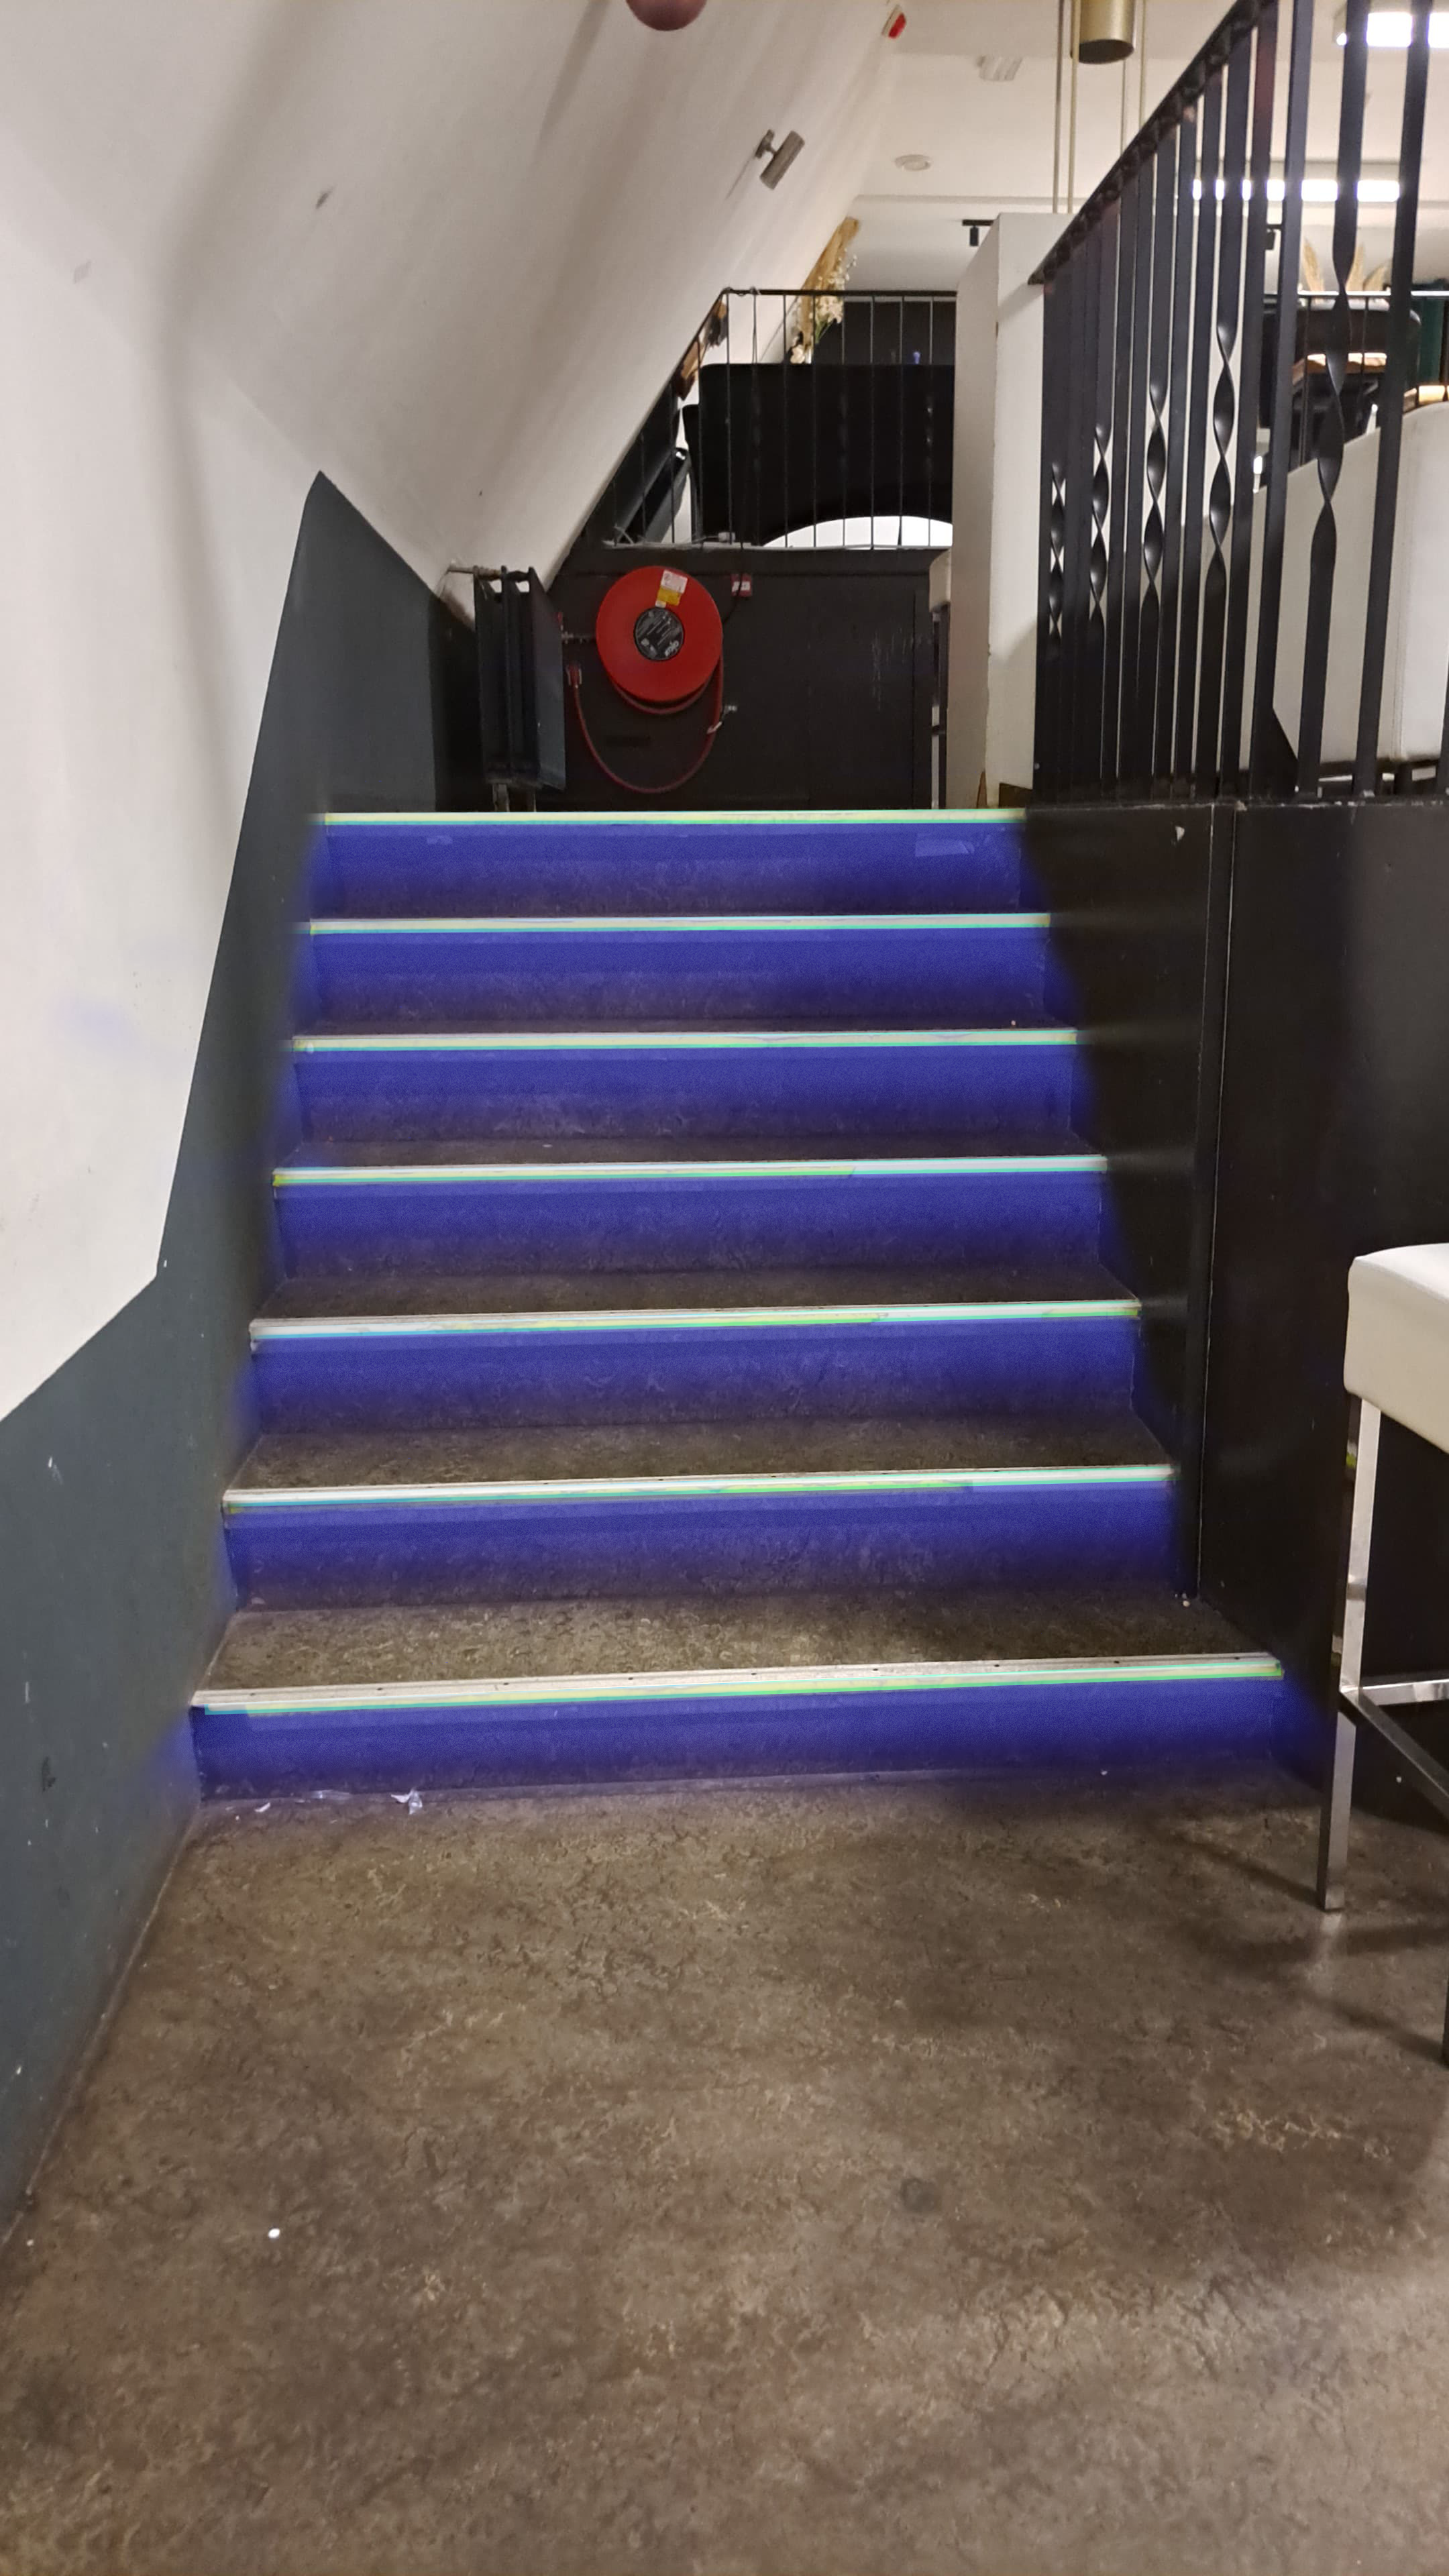
\includegraphics[width=.5\linewidth]{img/1892_trap_verlichting_render.png}
  \caption{Een schets van hoe de trap eruit komt te zien.}
  \label{fig:sub2}
\end{subfigure}
\caption{Een before and after tekening van de trap.}
\label{fig:test}
\end{figure}
\section{Requirements}

\subsection{Business Requirements:}
\begin{enumerate}
    \item Verbetering van de ambiance en veiligheid in het restaurant door middel van verbeterde verlichting onder de treden van de trappen.
    \item Implementatie van adresseerbare RGB LED-strips met waterdichte IP67 classificatie voor duurzaamheid.
    \item Creëren van een aantrekkelijke en robuuste verlichtingsoplossing die veel licht kan uitstralen.
    \item Ontwikkeling van een gebruiksvriendelijke app voor het aansturen van de LED-strips en het selecteren van verschillende effecten.
    \item Vooraf programmeren van de LED-strips met verschillende effecten voor eenvoudige installatie en gebruik.
\end{enumerate}

\subsection{User Requirements:}
\begin{enumerate}
    \item Toegang tot de app voor het eenvoudig aansturen van de LED-strips en het selecteren van gewenste effecten.
    \item Waterdichte en robuuste LED-strips die geschikt zijn voor gebruik onder de trappen.
    \item Mogelijkheid om de helderheid en kleuren van de LED's aan te passen via de app.
    \item Vereenvoudigde installatie en bediening van de LED-strips voor het personeel van het restaurant.
\end{enumerate}

\subsection{System Requirements:}
\begin{enumerate}
    \item LED-strips met adresseerbare RGB LED's en waterdichte IP67 classificatie.
    \item Ontwerp en fabricatie van printplaat inclusief behuizing voor de LED-strips.
    \item Implementatie van geaarde stopcontacten op aangegeven punten voor de voeding van de LED-strips.
    \item Nauwkeurige berekeningen van de benodigde stroom voor de LED-strips en controllers.
    \item Installatie van stroomtransformatoren voor het omzetten van 230V naar de benodigde spanning voor de controllers en LED's.
    \item Vooraf programmeren van de LED-strips met verschillende effecten voor eenvoudige installatie en gebruik.
\end{enumerate}
\section{Planning}
De planning voor het project zal continu worden besproken en afgestemd tussen Traccy Solutions en de eigenaar van 1892 Eten \& Drinken. Alle voortgang en taken zullen worden bijgehouden op een overzichtelijk platform waarin verschillende weergaven beschikbaar zijn, zoals lijsten en roadmaps.

\subsection{Overleg en Afstemming}
\begin{itemize}
    \item Regelmatige vergaderingen zullen worden gehouden om de voortgang van het project te bespreken en eventuele obstakels aan te pakken.
    \item Alle belanghebbenden zullen worden betrokken bij het besluitvormingsproces om ervoor te zorgen dat de vereisten en verwachtingen worden begrepen en nageleefd.
\end{itemize}

\subsection{Voortgangsregistratie}
\begin{itemize}
    \item Een overzichtelijk platform wordt opgezet om alle taken en voortgang van het project bij te houden.
    \item Verschillende weergaven, zoals lijsten en roadmaps, zullen beschikbaar zijn om de voortgang op verschillende niveaus te visualiseren.
\end{itemize}

\subsection{Deadlines}
\begin{itemize}
    \item Hoewel er op dit moment geen vaste deadlines zijn vastgesteld, wordt ernaar gestreefd het project binnen 3 maanden na aanvang ervan af te ronden.
    \item Indien nodig zullen tussentijdse mijlpalen worden vastgesteld om de voortgang te meten en ervoor te zorgen dat het project op schema blijft.
\end{itemize}

% \section{Interim Milestones}\label{Interim_milestones}

% Beschrijf in dit hoofdstuk welke producten je oplevert waar je met de uitvoering van de activiteiten naar
% toewerkt. Deze producten leiden dan samen naar het eindproduct. Voorbeelden van producten zijn:
% - Een verslag;
% - Tijdsplanning;
% - Een ontwerp
% - Een meetrapport
% - Een tekening;
% - Etc.

During the \textbf{PROJE4} course \textbf{Alset Innovations} will be designing a motor driver to drive a 78 Watts motor continuously. To achieve this a set of deliverables must be completed and delivered. These deliverables are mainly Reports and documents about the progress of the project. A detailed list is provided below.

\begin{itemize}
    \item Plan of Approach
        \begin{itemize}
            \item A detailed report about the Plan of Approach of \textbf{Alset Innovations}.
        \end{itemize}
    \item Intermediate Assessment 1
        \begin{itemize}
            \item Document in PDF format listing all of the detailed design requirements
            in relation to the software, including both interface and functionality
            requirements.
            \item Well documented and formatted code in original an pdf file formats.
            \item Summary of completed tests including hardware and software tests.
        \end{itemize}
    \item Intermediate Assessment 2
        \begin{itemize}
            \item Document in PDF format all of the detailed design requirements.
            in relation to the hardware.
            \item A zip file containing all PCB related design files as well as data-sheets for all active components.
            \item A well formatted pdf file containing pages showing both the schematic
            and the layout for the PCB design. The layout should be in a clear
            format such that it can be easily reviewed both from the top level
            design perspective and the individual layers.
            \item Maximum two page summary of the progress of the project, including
            the results of any tests on actual prototype hardware.
        \end{itemize}
    \item Final Assessment
        \begin{itemize}
            \item A detailed final report according to the provided template. In addition each student is required to write about their competencies.
        \end{itemize}
\end{itemize}
\section{Kosten}
Alle kosten zullen in detail uiteengezet worden in de bijgevoegde offerte. Wij zullen vooraf geen schatting maken van de arbeidsuren, maar deze zullen achteraf worden berekend en op de factuur worden vermeld. Daarom zal de offerte geen arbeidsuren bevatten.


\subsection{Transparantie}
Traccy Solutions zal transparant zijn over de kosten en zal ervoor zorgen dat de opdrachtgever volledig op de hoogte is van de financiële aspecten van het project. Eventuele wijzigingen in de kosten zullen tijdig worden gecommuniceerd en besproken.

% \subsection{Prototyping}


\subsection{Overschrijden budgettering}
Indien de kosten hoger blijken te zijn dan het oorspronkelijk geraamde bedrag, zal Traccy Solutions de opdrachtgever op de hoogte stellen van de situatie. In overleg met de opdrachtgever zal dan worden bepaald of het project wordt voortgezet met de eventueel hogere kosten of dat er wijzigingen moeten worden aangebracht om binnen het oorspronkelijke budget te blijven.
\section{Organisatie}
\subsection{1892 Eten \& Drinken}
De opdrachtgever voor dit project is Raymond Baboeram, eigenaar van 1892 Eten \& Drinken. Raymond zal fungeren als de belangrijkste contactpersoon voor communicatie en besluitvorming.

\subsection{Team Traccy Solutions}
Het team van Traccy Solutions bestaat uit de volgende leden, die elk verschillende verantwoordelijkheden dragen:

\begin{itemize}
    \item Laurens van der Drift (CEO): Laurens zal de leiding hebben over het project, inclusief planning, hardware en softwareontwikkeling, en de installatie van het systeem.
    \item Tommy Dobos: Tommy zal zich bezighouden met productontwerp, financiën, planning en de installatie van het systeem.
    \item Luuk van Kappel: Luuk zal zich richten op hardware- en softwareontwikkeling.
    \item Marnix Harmsen: Marnix zal zich toeleggen op softwareontwikkeling.
\end{itemize}

Elk teamlid brengt unieke vaardigheden en expertise naar het project, wat bijdraagt aan een uitgebalanceerd en effectief team.

%\include{chapters/Planning} %dit is project_activity geworden%
% \section{Software tools}
% De lezer leest in dit hoofdstuk hoe je de kwaliteit van de (tussen)producten uit de vorige paragraaf
% waarborgt. Dit kun je bijvoorbeeld beschrijven door:
% -
% - Of en in welke mate je gebruikmaakt van extern advies (bijv. iemand buiten je projectgroep die
% je (tussen)product controleert). Geef aan hoe je de feedback verwerkt;
% - Hoe je omgaat met regelgeving, veiligheid, programma van eisen etc;

% Te beschrijven welke software, materialen en andere hulpbronnen je gebruikt en hoet dit
% bijdraagt aan de kwaliteit van jullie projectresultaat.

% Om de kwaliteit voor het project te waarborgen zal er gebruik gemaakt worden van de software STM32CubeIDE, waarmee de stm32-microcontroller geprogrammeerd kan worden. De stm32-chip is gebruikelijk in de industrie, vanwege zijn manier van programmeren, zoals het instellen van de GPIO en klokfrequenties. Bovendien zou het realtime simulatiepakket Caspoc gebruikt kunnen worden. Hiermee kan de werking en aansturing van de motordriver getest worden. Daarnaast wordt KiCad 7.0 gebruikt voor het ontwerpen van PCB's. Kicad is opensource en beschikt over de functies om een PCB te ontwerpen voor de motordriver. Het bestellen van de PCB wordt bij Eurocircuits gedaan, vanwege afspraken die school heeft gemaakt. \\
% Voor het aanschaffen van materialen zijn bedrijven zoals Conrad, Farnell, Texas Instruments en Mouser geschikt, omdat zij beschikken over een aanbod van hardware voor de motordriver.\\
% Voor het vragen van advies kan er terecht bij:
% \begin{itemize}
%   \item Jesse op den Brouw: C-programmeur
%   \item Stephen O'Loughlin: algemeen advies
%   \item Ad van den Bergh: programmeur
%   \item Diëgo Zuidervliet: kennis voor het aansturen van motordrivers
%   \item Paul Witte: PCB-designer
% \end{itemize}
% Voor het controleren van de (tussen)producten worden assesments gegeven met de docenten die hiervoor een aantal punten geven. Bovendien wordt er elke week een vergadering georganiseerd, waarbij de begeleider betrokken is en eventueel feedback kan geven.\\
% Het ontvangen van feedback wordt meegenomen in de toekomstige activiteiten om zo tot een beter ontwerp te komen. Daarnaast hoeft er geen rekening gehouden te worden met de regelgeving, omdat het eindproduct voor eigengebruik is. Voor de veiligheid moeten componenten gekoeld worden en niet kunnen ontploffen. Het eindproduct zal de minimale eisen hebben volgens het programma van eisen, maar de mogelijkheid bestaat dat er extra functies worden toegevoegd.\\
% Alle bovengenoemde producten moeten zorgen dat er een functionele motordriver ontworpen kan worden.



To ensure the quality of the project, the following software and resources will be utilized:

\begin{itemize}
  \item \textbf{STM32CubeIDE}: This software will be used for programming the STM32 microcontroller, which is commonly used in the industry due to its programming capabilities such as configuring GPIO and clock frequencies.
  \item \textbf{Caspoc Real-time Simulation Package}: This tool will be employed to test the operation and control of the motor driver in real-time simulations.
  \item \textbf{KiCad 8.0 and Altium Designer}: This will be utilized for designing and testing PCBs for the motor driver.
   \item \textbf{Arduino IDE}: Open source software for programming microcontrollers, such as ESP32 and the Arduino.
   \item \textbf{Visual Studio Code}: This will be used for writing in programming languages.
  \item \textbf{Eurocircuits}: PCB manufacturing will be done through Eurocircuits as per the agreements made by the school.
\end{itemize}

For procurement of materials, companies such as Conrad, Farnell, Texas Instruments, and Mouser will be considered due to their hardware offerings for the motor driver.

Expert advice can be sought from the following individuals:
\begin{itemize}
  \item Jesse op den Brouw: C programmer
  \item Stephen O'Loughlin: General advice
  \item Ad van den Bergh: Programmer
  \item Diëgo Zuidervliet: Expertise in motor driver control
  \item Paul Witte: PCB designer
\end{itemize}

Assessments will be conducted by instructors to evaluate the (intermediate) products. Additionally, weekly meetings will be held involving the supervisor to provide feedback.
Feedback received will be incorporated into future activities to enhance the design. 

% Regulatory considerations are not necessary as the end product is for personal use. However, components must be cooled for safety, and precautions must be taken to prevent explosions. The final product will meet the minimum requirements outlined in the specifications, with the possibility of additional features being added.


% \phantomsection
\addcontentsline{toc}{section}{Referenties}
\printbibliography
\end{document}
